%%%%%%%%%%%%%%%%%%%%%%%%%%%%%%%%%%%%%%%%%%
\fe{\section{Maillage}}{\section{Meshing}}
\label{maillage}
%%%%%%%%%%%%%%%%%%%%%%%%%%%%%%%%%%%%%%%%%%

\begin{frame}{\fe{Géométrie}{Geometry}}
  \begin{itemize}
    \item \fe{Dimensions de la pièce}{Dimensions of the part}\\
    \begin{center}
      \tiny
      \begin{tikzpicture}
        \node[anchor=south west,inner sep=0] (image) at (0,0)
        {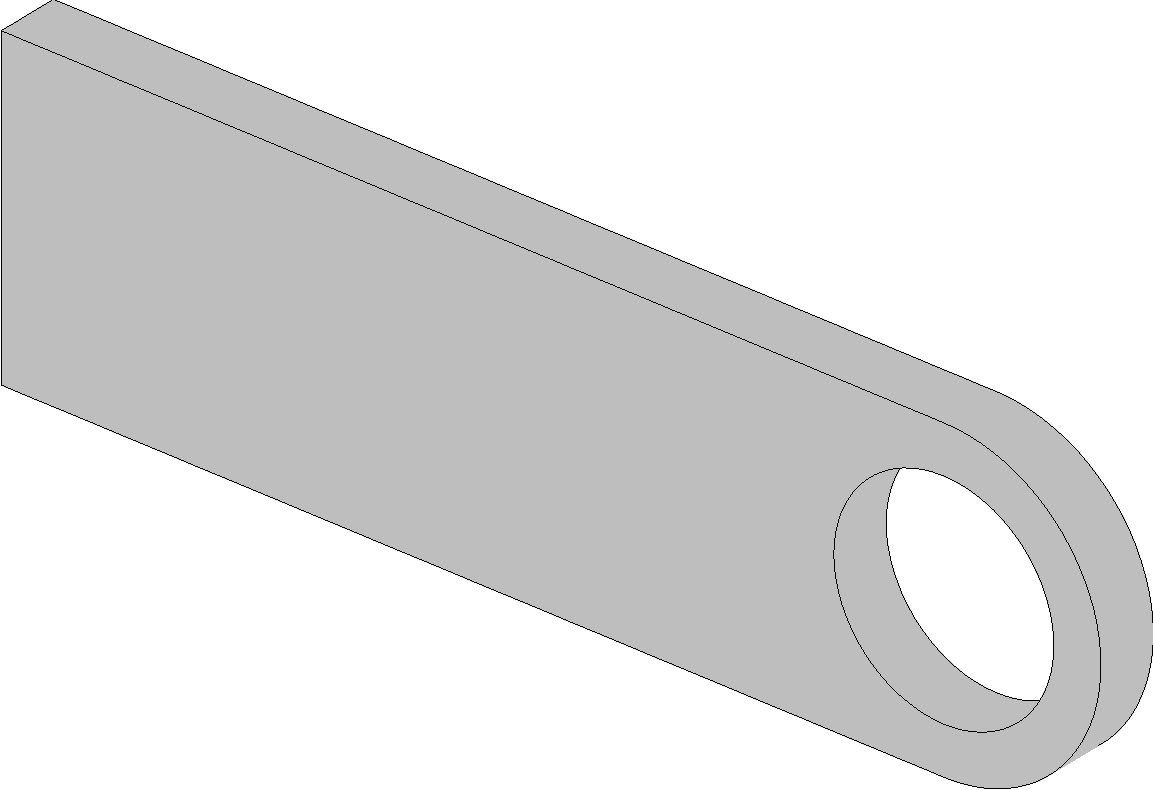
\includegraphics[width=7cm]{images/exo/1.2_geometrie}};
        \begin{scope}[x={(image.south east)},y={(image.north west)}]
  %        \grille
          \draw[latex-latex,thick,<->] (0,0.45) -- (0.82,-0.05) node[midway,fill=white]{30~cm};
          \draw[latex-latex,thick,<->] (-0.06,0.51) -- (-0.06,0.96) node[midway,fill=white]{10~cm};
          \draw[thick,<->] (0,1) -- (0.05,1.05);
          \draw (0.07,1.1) node[anchor=north west] {2~cm};
          \draw[thick,->] (0.82,0.25) -- (0.75,0.4);
          \draw (0.75,0.4) node[anchor=south east] {3,5~cm};
          \draw[dotted,thick] (0.82,-0.1) -- (0.82,0.3);
        \end{scope}
      \end{tikzpicture}
    \end{center}
    \normalsize
  \end{itemize}
\end{frame}

\begin{frame}{\fe{1.1 Maillage non structuré}{1.1 Unstructured mesh}}
  \begin{itemize}
    \item \fe{Objectif : créer un \g{maillage paramétré} de la structure}
             {Objective: to create a \g{parametered mesh} of the structure}
    \begin{itemize}
      \item[] $\Rightarrow$ \fe{maillage non structuré}{unstructured grid}
      \item[] $\Rightarrow$ \fe{paramètre : taille de maille globale}
                              {parameter: average element size}
      \item[] $\Rightarrow$ \fe{éléments triangles/tétraèdres}{triangles/tetrahedra elements}
      \item[]
    \end{itemize}
    \item \fe{Méthode :}{Method:}
    \begin{enumerate}
      \item \fe{placer des points guides}{define the main points}
      \item \fe{mailler le contour fermé}{mesh the closed border} 
      \item \fe{mailler la surface par remplissage}{mesh the internal surface by filling}
      \item \fe{mailler le volume par extrusion}{mesh the volume by extrusion}
    \end{enumerate}
  \end{itemize}
\end{frame}

\begin{frame}{\fe{1.1 Maillage non structuré}{1.1 Unstructured mesh}}
  \begin{itemize}
    \item \fe{Options générales et paramètres}{General options and parameters}
    \lstinputlisting[language=gibiane, firstline=33, lastline=40]{dgibi/formation_debutant_1_maillage.dgibi}
    \lstinputlisting[language=gibiane, firstline=56, lastline=57]{dgibi/formation_debutant_1_maillage.dgibi}
    \item[] \violet{\emph{\fe{Nouveaux objets :}{New objects:} ENTIER, FLOTTANT, MOT}}
  \end{itemize}
\end{frame}

\begin{frame}{\fe{1.1 Maillage non structuré}{1.1 Unstructured mesh}}
  \begin{itemize}
    \item \fe{Création de points}{Points creation}
    \lstinputlisting[language=gibiane, firstline=59, lastline=69]{dgibi/formation_debutant_1_maillage.dgibi}
    \item[] \violet{\emph{\fe{Nouveaux objets :}{New objects:} POINT}}
  \end{itemize}
\end{frame}

\begin{frame}{\fe{1.1 Maillage non structuré}{1.1 Unstructured mesh}}
  \begin{itemize}
    \item \fe{Maillage des lignes et de contours fermés}{Meshing lines and closed contours}
    \lstinputlisting[language=gibiane, firstline=71, lastline=73]{dgibi/formation_debutant_1_maillage.dgibi}
    \lstinputlisting[language=gibiane, firstline=78, lastline=84]{dgibi/formation_debutant_1_maillage.dgibi}
    \onslide<2->{
      \lstinputlisting[language=gibiane, firstline=86, lastline=86]{dgibi/formation_debutant_1_maillage.dgibi}
      \begin{textblock*}{5cm}(8.1cm,-2.6cm)
        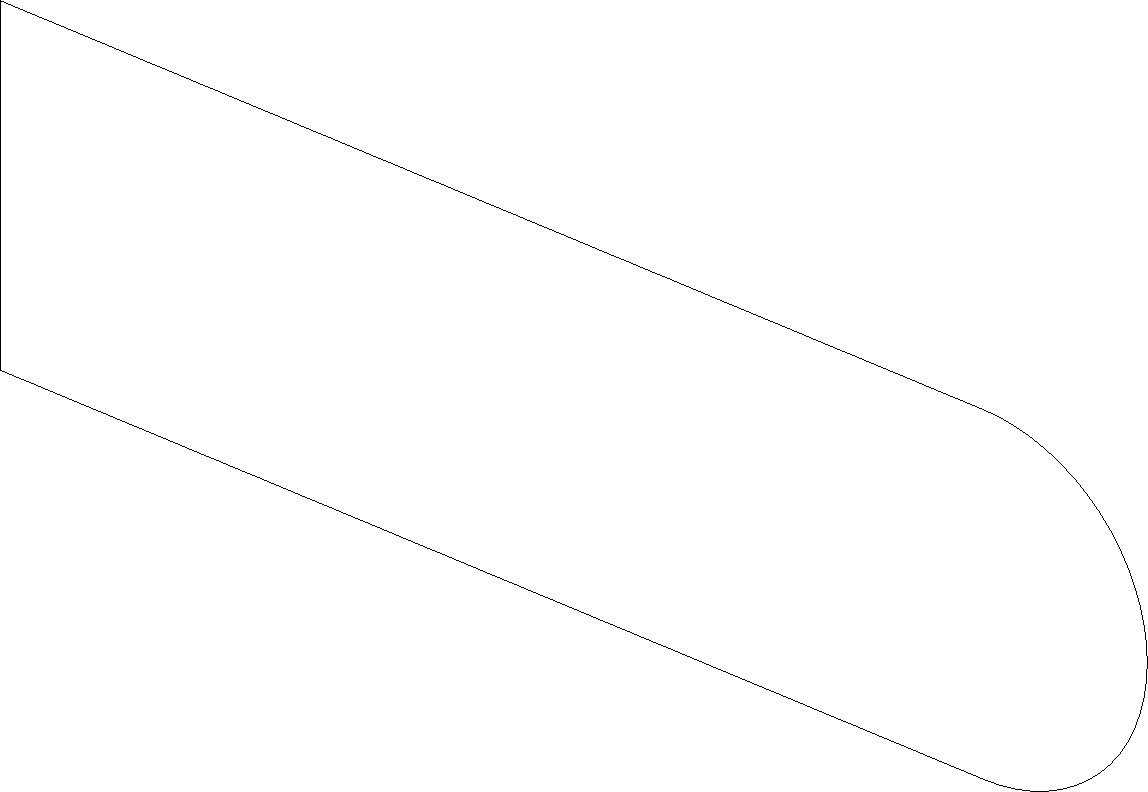
\includegraphics[width=4cm]{images/exo/1.1_maillage_tetra.01}
      \end{textblock*}}
    \onslide<3->{
      \footnotesize
      \avous{\fe{Maillage du cercle de centre p6}{Meshing the circle with center p6}}
      \normalsize}
    \onslide<4->{
      \lstinputlisting[language=gibiane, firstline=88, lastline=89]{dgibi/formation_debutant_1_maillage.dgibi}
      \lstinputlisting[language=gibiane, firstline=91, lastline=91]{dgibi/formation_debutant_1_maillage.dgibi}
      \begin{textblock*}{5cm}(8.1cm,-2.5cm)
        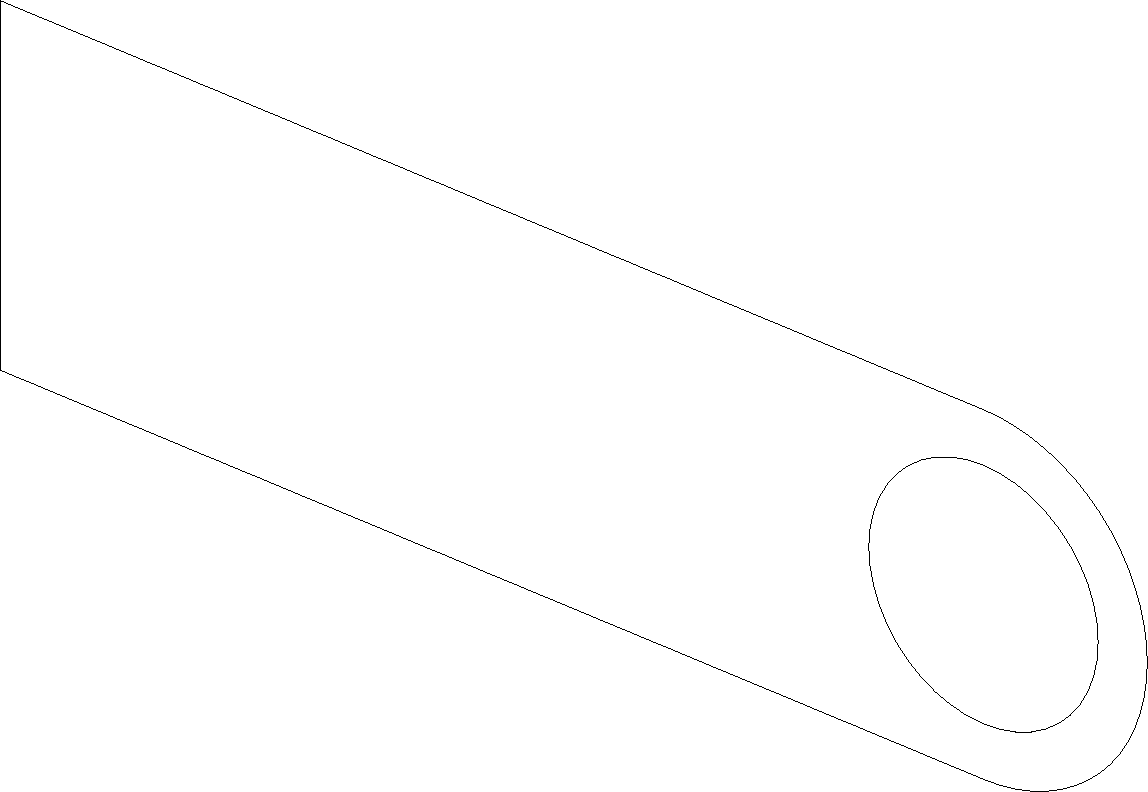
\includegraphics[width=4cm]{images/exo/1.1_maillage_tetra.02}
      \end{textblock*}}
    \item[] \violet{\emph{\fe{Nouveaux objets :}{New objects:} MAILLAGE}}
  \end{itemize}
\end{frame}

\begin{frame}{\fe{1.1 Maillage non structuré}{1.1 Unstructured mesh}}
  \begin{itemize}
    \item \fe{Maillage de la surface (maillage libre depuis le contour fermé)}
             {Surface meshing (unstructured mesh inside the closed contour)}
    \lstinputlisting[language=gibiane, firstline=93, lastline=94]{dgibi/formation_debutant_1_maillage.dgibi}
    \onslide<2->{
      \lstinputlisting[language=gibiane, firstline=96, lastline=96]{dgibi/formation_debutant_1_maillage.dgibi}}
    \onslide<2-3>{
      \begin{textblock*}{5cm}(8.1cm,-1.cm)
        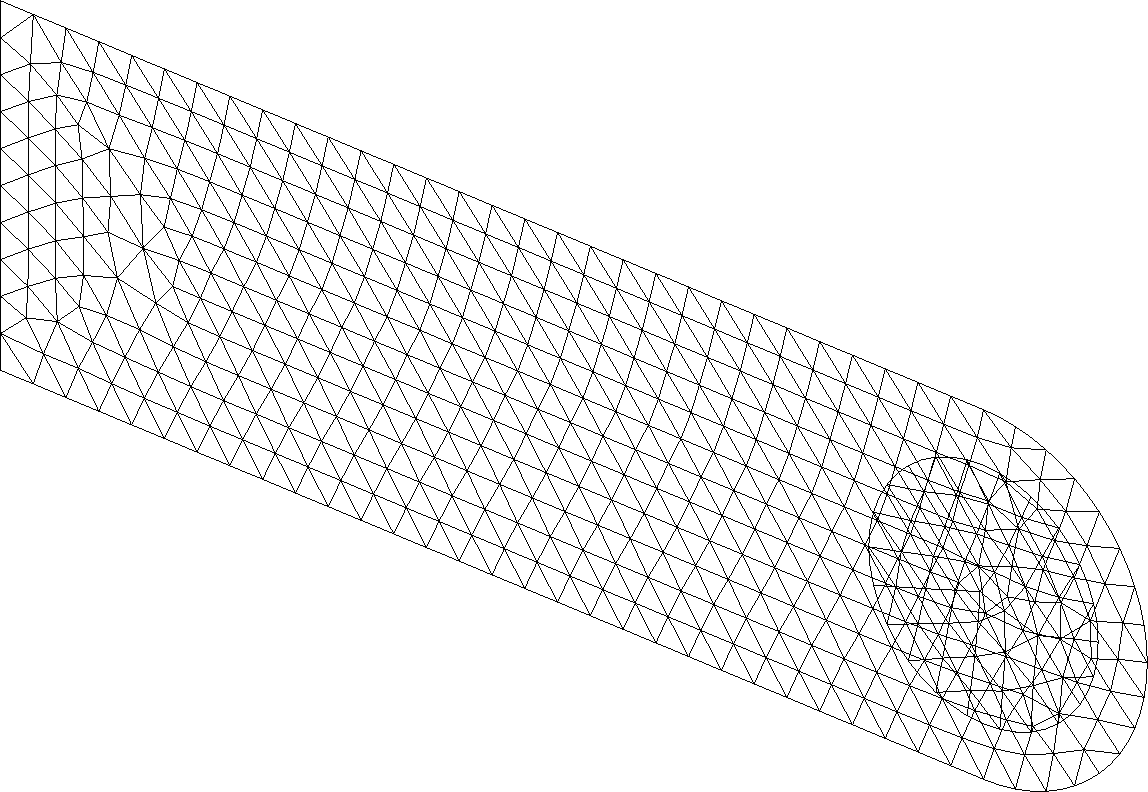
\includegraphics[width=4cm]{images/exo/1.1_maillage_tetra.03}
      \end{textblock*}}
    \onslide<3->{
      \lstinputlisting[language=gibiane, firstline=98, lastline=99]{dgibi/formation_debutant_1_maillage.dgibi}}
    \onslide<4->{
      \lstinputlisting[language=gibiane, firstline=101, lastline=101]{dgibi/formation_debutant_1_maillage.dgibi}
      \begin{textblock*}{5cm}(8.1cm,-2.5cm)
        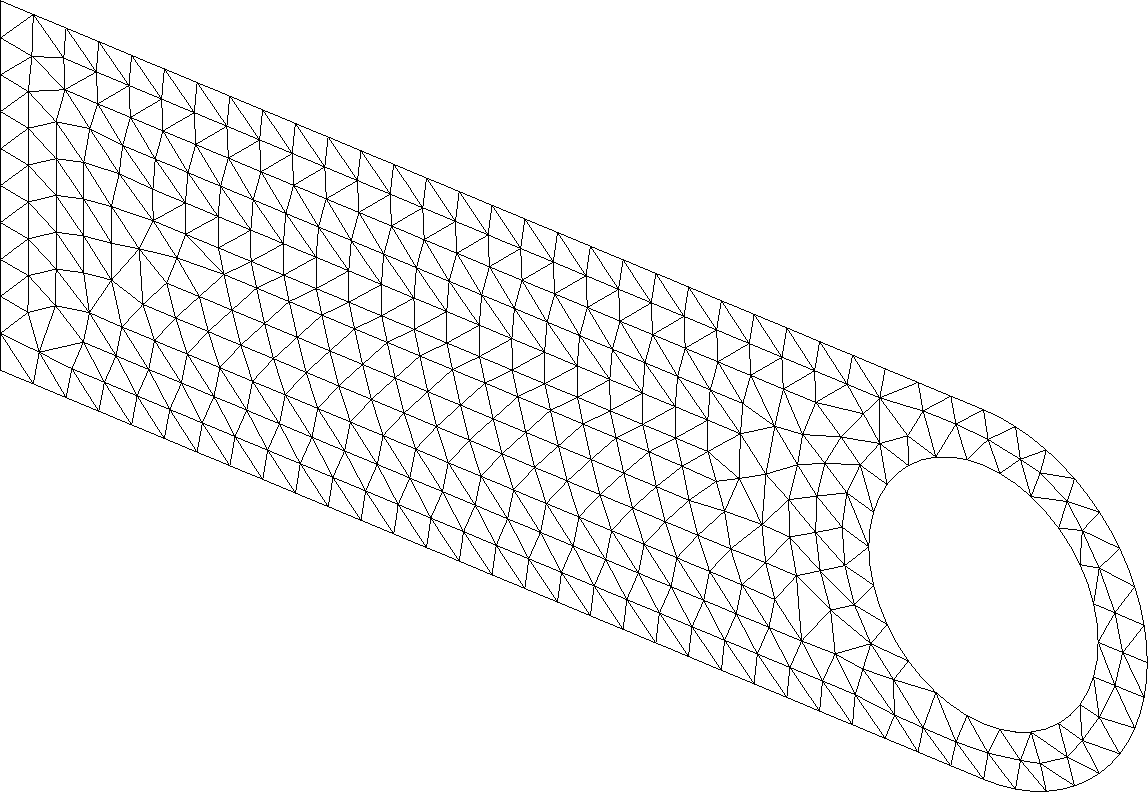
\includegraphics[width=4cm]{images/exo/1.1_maillage_tetra.04}
      \end{textblock*}}
    \item<5->\fe{Maillage du volume}{Meshing the volume}\\
    \onslide<5->{
      \footnotesize
      \avous{\fe{Mailler le volume par translation (voir : VOLU)}{Mesh the volume by translation (see: VOLU)}}
      \normalsize}
    \onslide<6->{
    \lstinputlisting[language=gibiane, firstline=103, lastline=104]{dgibi/formation_debutant_1_maillage.dgibi}}
    \onslide<6->{
      \lstinputlisting[language=gibiane, firstline=106, lastline=106]{dgibi/formation_debutant_1_maillage.dgibi}}
    \onslide<6>{
      \begin{textblock*}{5cm}(8.1cm,-2.cm)
        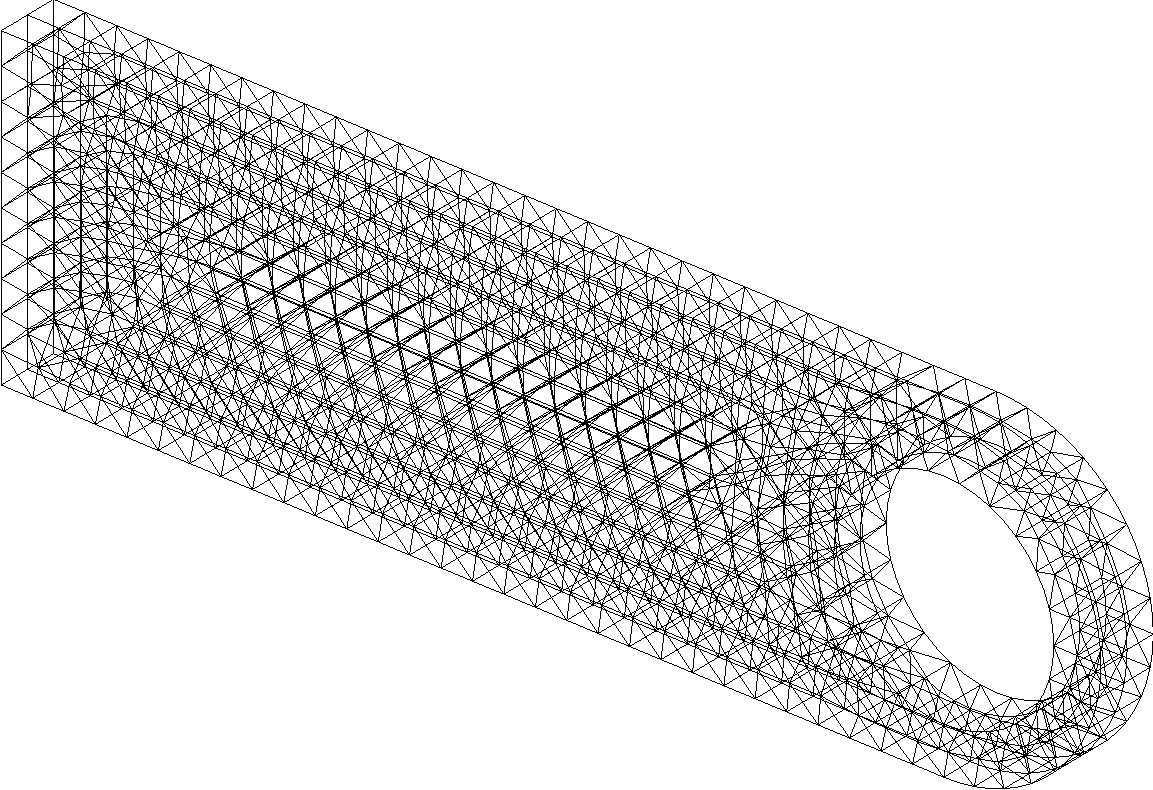
\includegraphics[width=4cm]{images/exo/1.1_maillage_tetra.05}
      \end{textblock*}}
    \onslide<7->{
      \lstinputlisting[language=gibiane, firstline=107, lastline=107]{dgibi/formation_debutant_1_maillage.dgibi}
      \begin{textblock*}{5cm}(8.1cm,-2.5cm)
        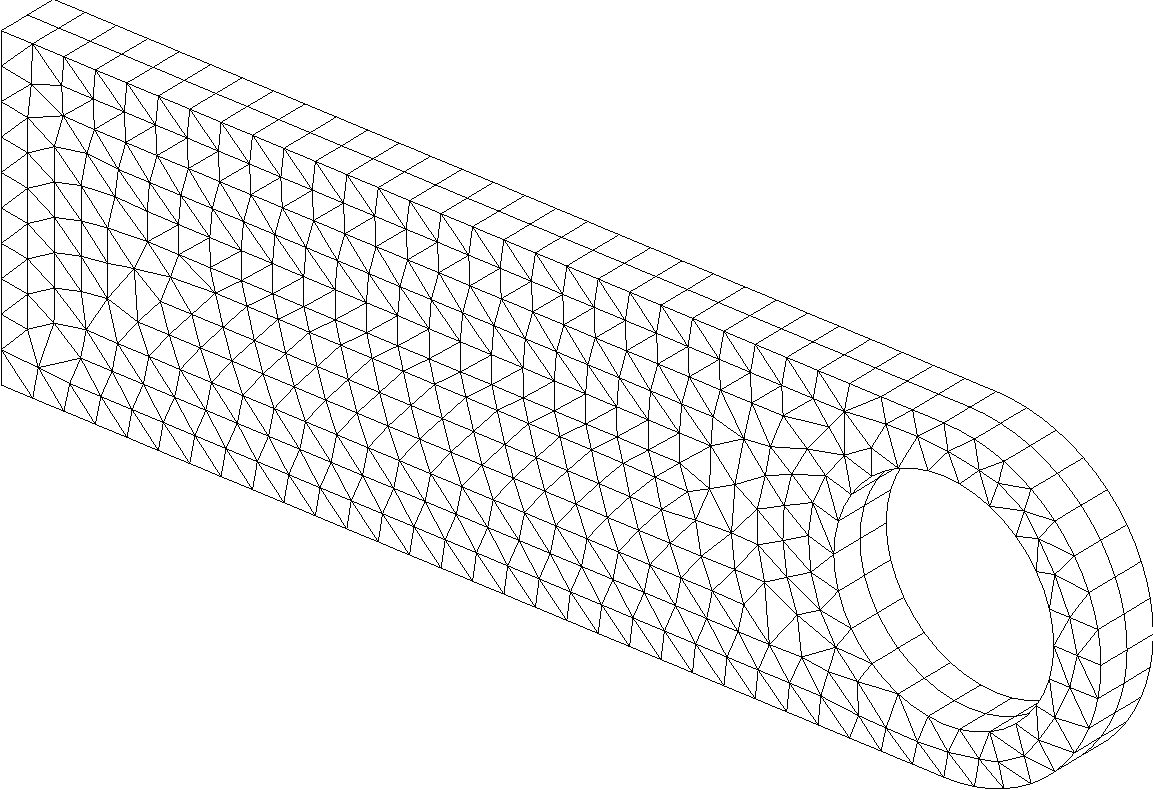
\includegraphics[width=4cm]{images/exo/1.1_maillage_tetra.06}
      \end{textblock*}}
    \item<8->\fe{Le maillage est fait de prismes !}{The mesh is made of prisms!}
  \end{itemize}
\end{frame}

\begin{frame}{\fe{1.1 Maillage non structuré}{1.1 Unstructured mesh}}
  \begin{itemize}
    \item \fe{Modification du type d'éléments}{Changing the type of elements}
    \lstinputlisting[language=gibiane, firstline=109, lastline=111]{dgibi/formation_debutant_1_maillage.dgibi}
    \lstinputlisting[language=gibiane, firstline=113, lastline=113]{dgibi/formation_debutant_1_maillage.dgibi}
    \begin{textblock*}{5cm}(8.1cm,-2.4cm)
      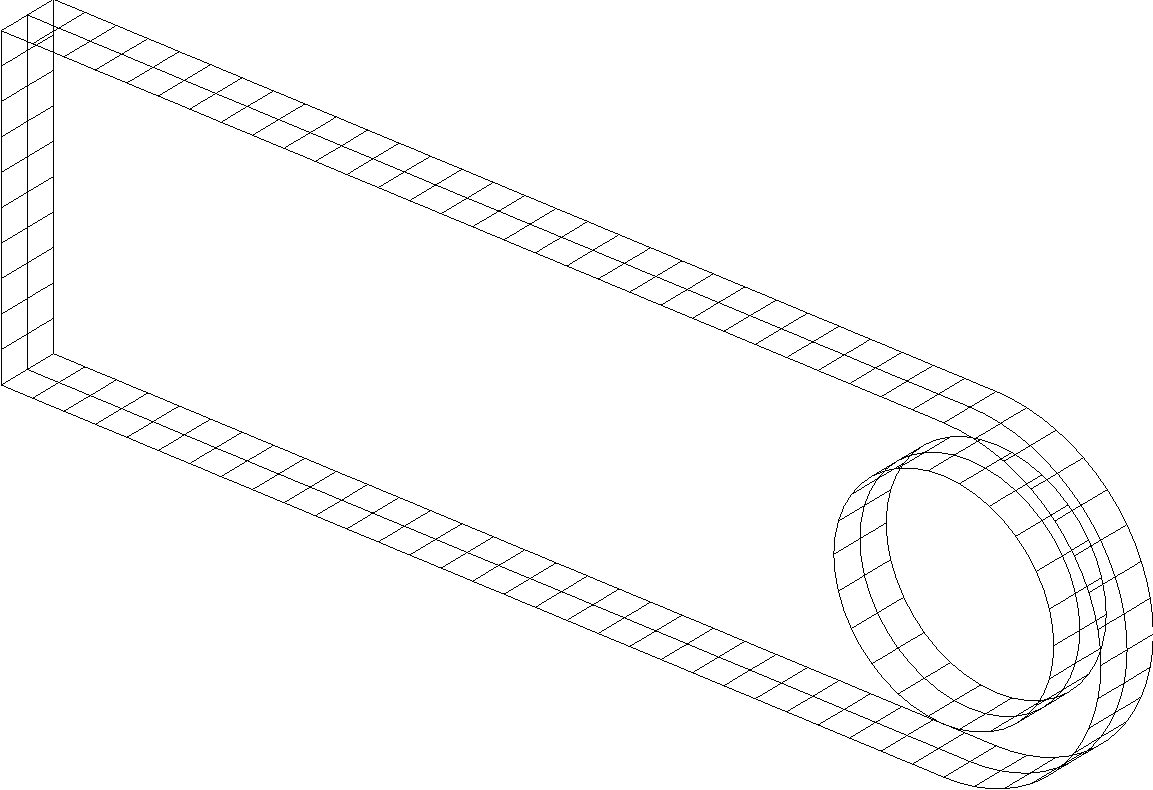
\includegraphics[width=4cm]{images/exo/1.1_maillage_tetra.07}
    \end{textblock*}
    \onslide<2->{
      \lstinputlisting[language=gibiane, firstline=115, lastline=117]{dgibi/formation_debutant_1_maillage.dgibi}}
    \onslide<3->{
      \lstinputlisting[language=gibiane, firstline=119, lastline=119]{dgibi/formation_debutant_1_maillage.dgibi}
      \begin{textblock*}{5cm}(8.1cm,-2.4cm)
        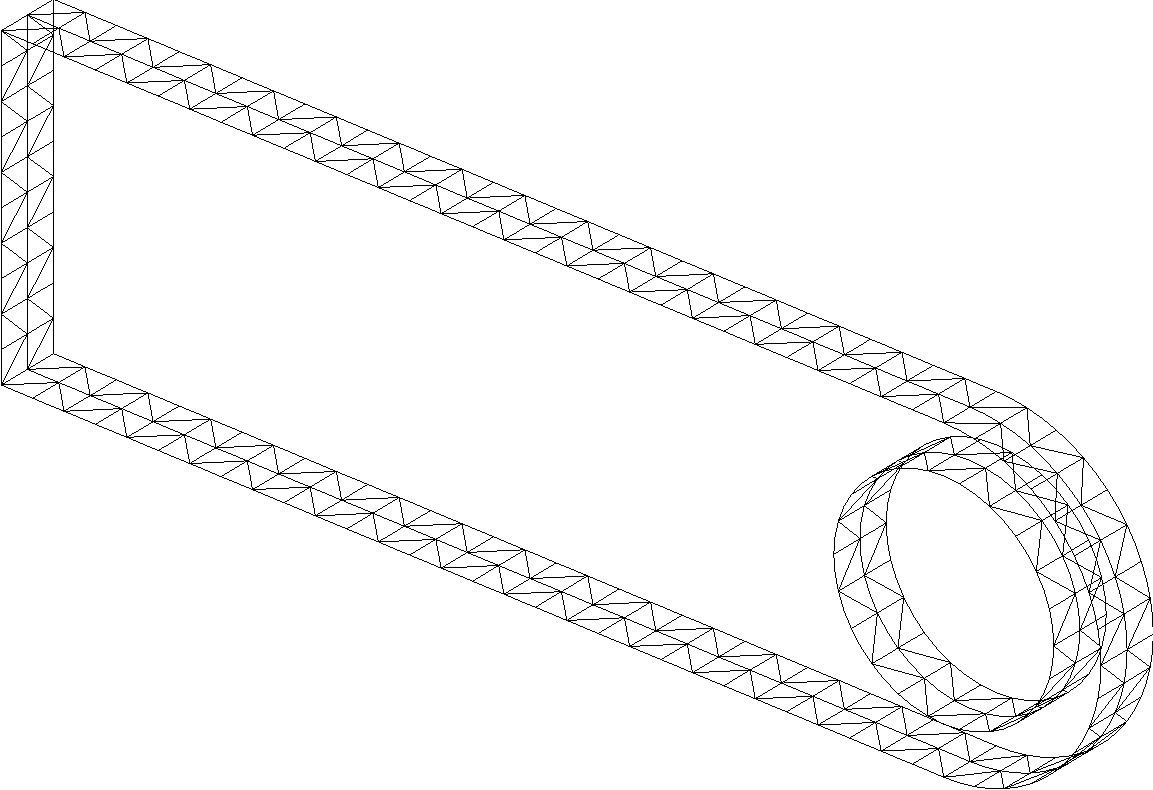
\includegraphics[width=4cm]{images/exo/1.1_maillage_tetra.08}
      \end{textblock*}}
    \onslide<4->{
      \footnotesize
      \avous{\fe{Mailler le volume dans la surface enveloppe (voir : VOLU)}
                {Mesh the volume inside the enveloppe (see: VOLU)}}
      \normalsize}
    \onslide<5->{
      \lstinputlisting[language=gibiane, firstline=121, lastline=123]{dgibi/formation_debutant_1_maillage.dgibi}
      \lstinputlisting[language=gibiane, firstline=125, lastline=125]{dgibi/formation_debutant_1_maillage.dgibi}
      \begin{textblock*}{5cm}(8.1cm,-1.8cm)
        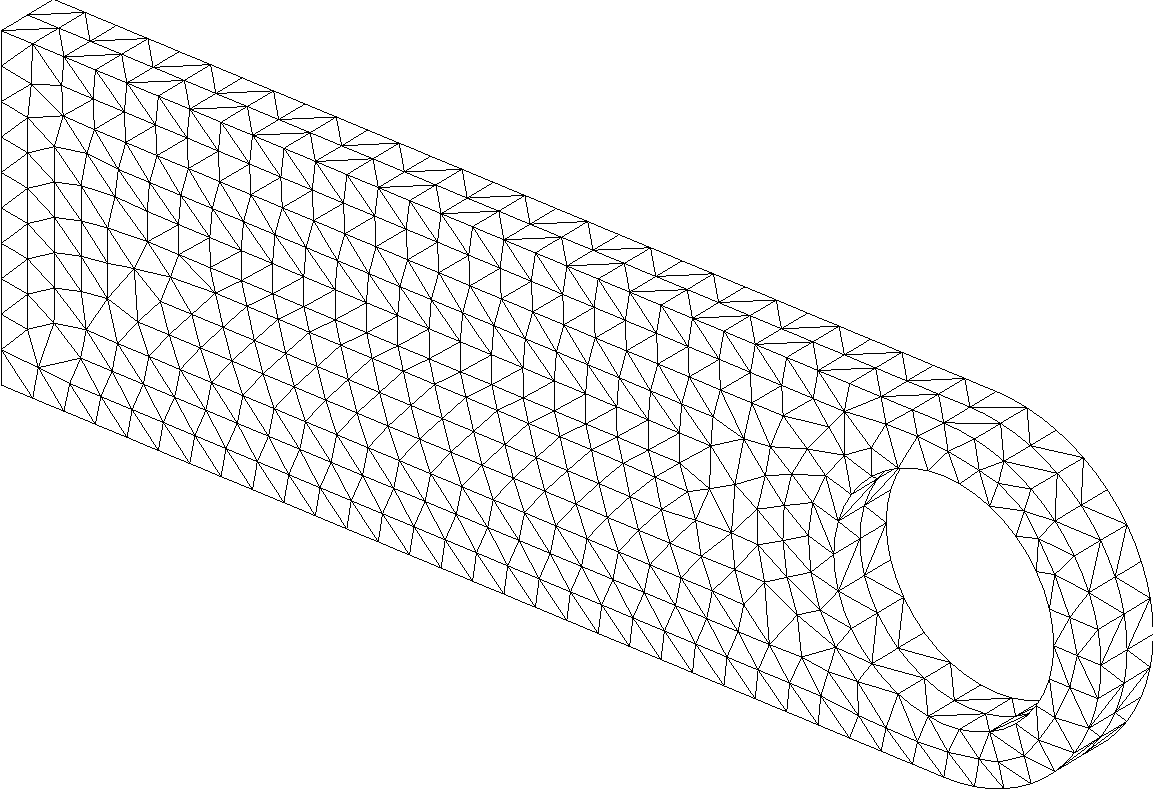
\includegraphics[width=4cm]{images/exo/1.1_maillage_tetra.09}
      \end{textblock*}}
  \end{itemize}
\end{frame}

\begin{frame}{\fe{1.2 Maillage structuré}{1.2 Structured mesh}}
  \begin{itemize}
    \item \fe{Objectif : créer un \g{maillage paramétré} de la structure}
            {Objective: to create a \g{parametered mesh} of the structure}
    \begin{itemize}
      \item[] $\Rightarrow$ \fe{maillage structuré}{structured grid}
      \item[] $\Rightarrow$ \fe{paramètre : nombre d'éléments sur les arêtes}
                              {parameter: number of elements on the edges}
      \item[] $\Rightarrow$ \fe{éléments quadrangles/hexaèdres}{quadrangles/hexahedra elements}
      \item[]
    \end{itemize}
    \item \fe{Méthode :}{Method:}
    \begin{enumerate}
      \item \fe{placer des points guides}{define the main points}
      \item \fe{mailler des lignes opposées}{mesh opposed lines}
      \item \fe{mailler des surfaces réglées}{mesh ruled surfaces}
      \item \fe{mailler le volume par extrusion}{mesh the volume by extrusion}
    \end{enumerate}
  \end{itemize}
\end{frame}

\begin{frame}{\fe{1.2 Maillage structuré}{1.2 Structured mesh}}
  \begin{itemize}
    \item \fe{Options et paramètres}{Options and parameters}
    \lstinputlisting[language=gibiane, firstline=143, lastline=145]{dgibi/formation_debutant_1_maillage.dgibi}
    \lstinputlisting[language=gibiane, firstline=150, lastline=152]{dgibi/formation_debutant_1_maillage.dgibi}
    \item<2->\fe{Maillage surfacique par translation}{Surface mesh by translation}
    \lstinputlisting[language=gibiane, firstline=154, lastline=158]{dgibi/formation_debutant_1_maillage.dgibi}
    \lstinputlisting[language=gibiane, firstline=160, lastline=160]{dgibi/formation_debutant_1_maillage.dgibi}
    \onslide<2->{
      \begin{textblock*}{5cm}(8.1cm,-2.7cm)
        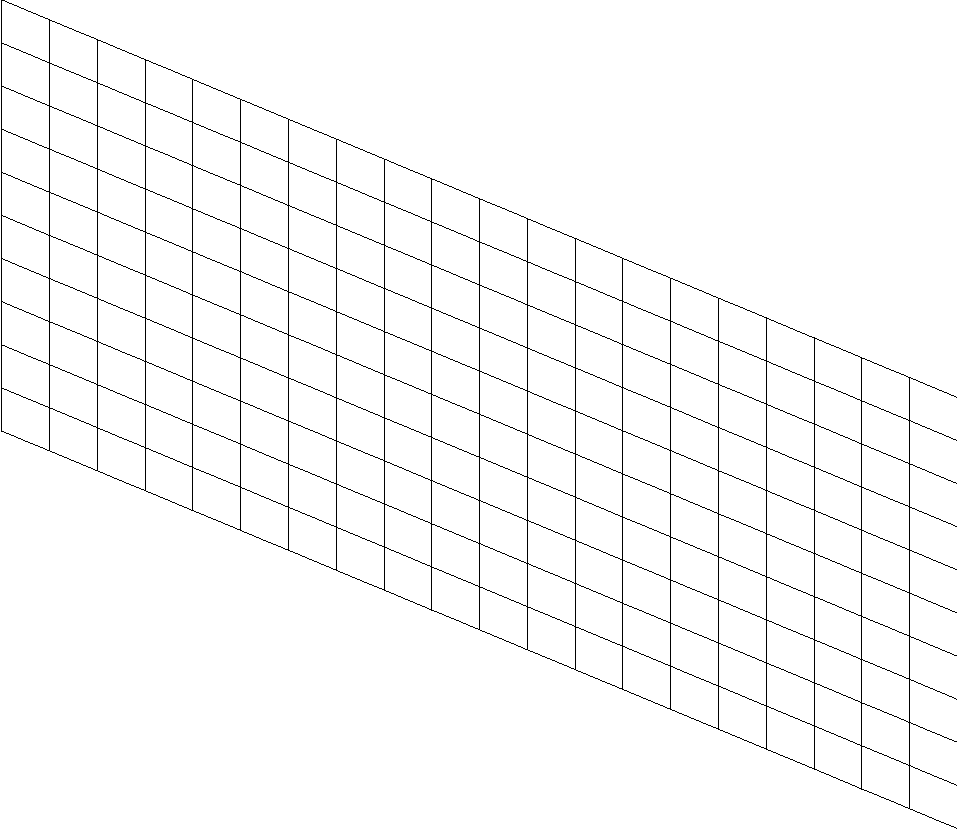
\includegraphics[width=4cm]{images/exo/1.2_maillage_hexa.1}
      \end{textblock*}}
  \end{itemize}
\end{frame}

\begin{frame}{\fe{1.2 Maillage structuré}{1.2 Structured mesh}}
  \begin{itemize}
    \item \fe{Récupération de sous zones}{Subzone recovery}
    \lstinputlisting[language=gibiane, firstline=162, lastline=166]{dgibi/formation_debutant_1_maillage.dgibi}
    \item<2->\fe{Maillage de la surface autour du trou}{Surface mesh around the hole}
    \lstinputlisting[language=gibiane, firstline=167, lastline=171]{dgibi/formation_debutant_1_maillage.dgibi}
    \onslide<3->{
      \footnotesize
      \avous{\fe{Mailler le cercle du trou par PROJection de \kw{lig1}}
                {Mesh the circle of the hole by PROJection of \kw{lig1}}}
      \normalsize}
    \onslide<4->{
    \lstinputlisting[language=gibiane, firstline=172, lastline=174]{dgibi/formation_debutant_1_maillage.dgibi}
    \lstinputlisting[language=gibiane, firstline=176, lastline=176]{dgibi/formation_debutant_1_maillage.dgibi}
      \begin{textblock*}{5cm}(9cm,-4.1cm)
        \begin{tikzpicture}
          \node[anchor=south west,inner sep=0] (image) at (0,0)
          {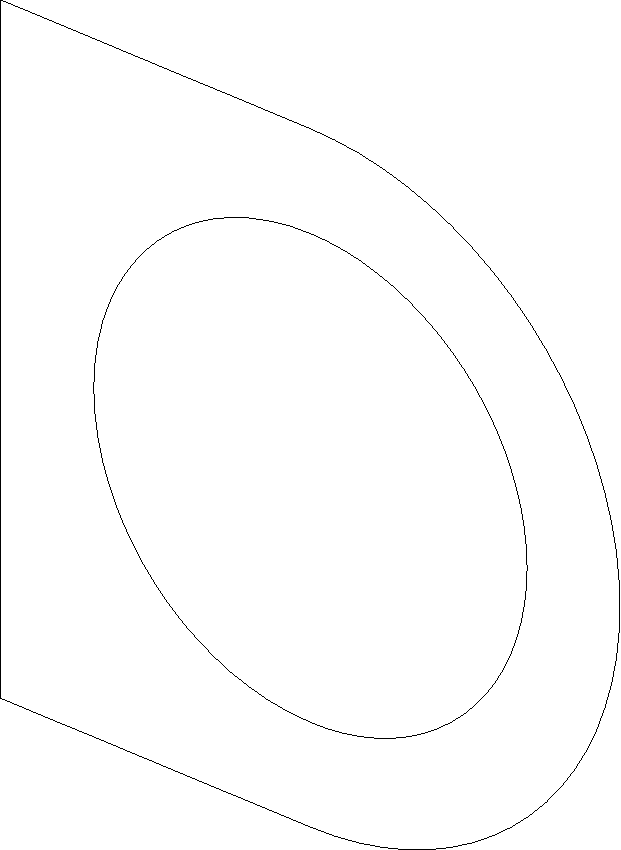
\includegraphics[width=3cm]{images/exo/1.2_maillage_hexa.2}};
          \begin{scope}[x={(image.south east)},y={(image.north west)}]
            \tiny
            \draw (0.02,0.2) node[anchor=west] {\kw{lig1}};
            \draw (0.3,0.3) node[anchor=west] {\kw{cin}};
          \end{scope}
        \end{tikzpicture}
      \end{textblock*}}
  \end{itemize}
\end{frame}

\begin{frame}{\fe{1.2 Maillage structuré}{1.2 Structured mesh}}
  \begin{itemize}
    \item \fe{Maillage de la surface réglée}{Meshing the ruled surface}\\
    \footnotesize
    \avous{\fe{Mailler la surface réglée entre \kw{cin} et \kw{lig1}\\
         \quad avec 3 éléments (voir : REGL)}
              {Mesh the ruled surface between \kw{cin} and \kw{lig1}\\
        \qquad with 3 elements (see: REGL)}}
    \normalsize
    \onslide<1-2>{
      \begin{textblock*}{5cm}(9cm,-2cm)
        \begin{tikzpicture}
          \node[anchor=south west,inner sep=0] (image) at (0,0)
          {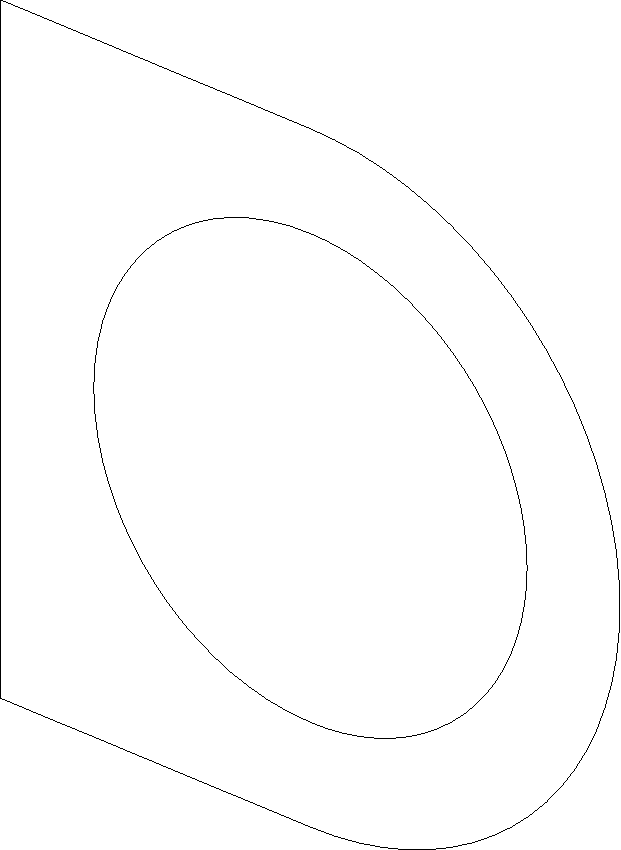
\includegraphics[width=3cm]{images/exo/1.2_maillage_hexa.2}};
          \begin{scope}[x={(image.south east)},y={(image.north west)}]
            \tiny
            \draw (0.02,0.2) node[anchor=west] {\kw{lig1}};
            \draw (0.3,0.3) node[anchor=west] {\kw{cin}};
          \end{scope}
        \end{tikzpicture}
      \end{textblock*}}
      \onslide<2->{
      \lstinputlisting[language=gibiane, firstline=178, lastline=182]{dgibi/formation_debutant_1_maillage.dgibi}}
    \onslide<3->{
      \lstinputlisting[language=gibiane, firstline=184, lastline=184]{dgibi/formation_debutant_1_maillage.dgibi}
      \begin{textblock*}{5cm}(8.1cm,-2cm)
        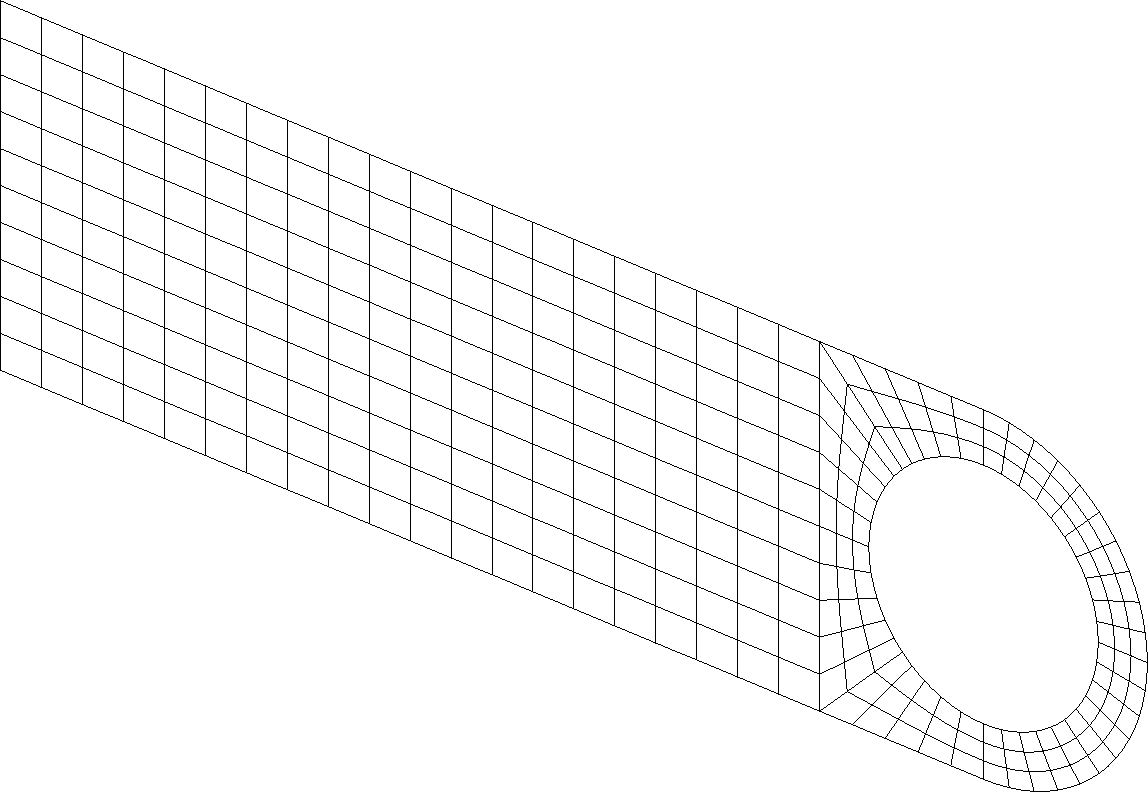
\includegraphics[width=4cm]{images/exo/1.2_maillage_hexa.3}
      \end{textblock*}}
    \item<4->\fe{Maillage du volume par translation}{Meshing the volume by translation}
    \lstinputlisting[language=gibiane, firstline=186, lastline=187]{dgibi/formation_debutant_1_maillage.dgibi}
    \lstinputlisting[language=gibiane, firstline=189, lastline=189]{dgibi/formation_debutant_1_maillage.dgibi}
    \begin{textblock*}{5cm}(8.1cm,-2cm)
      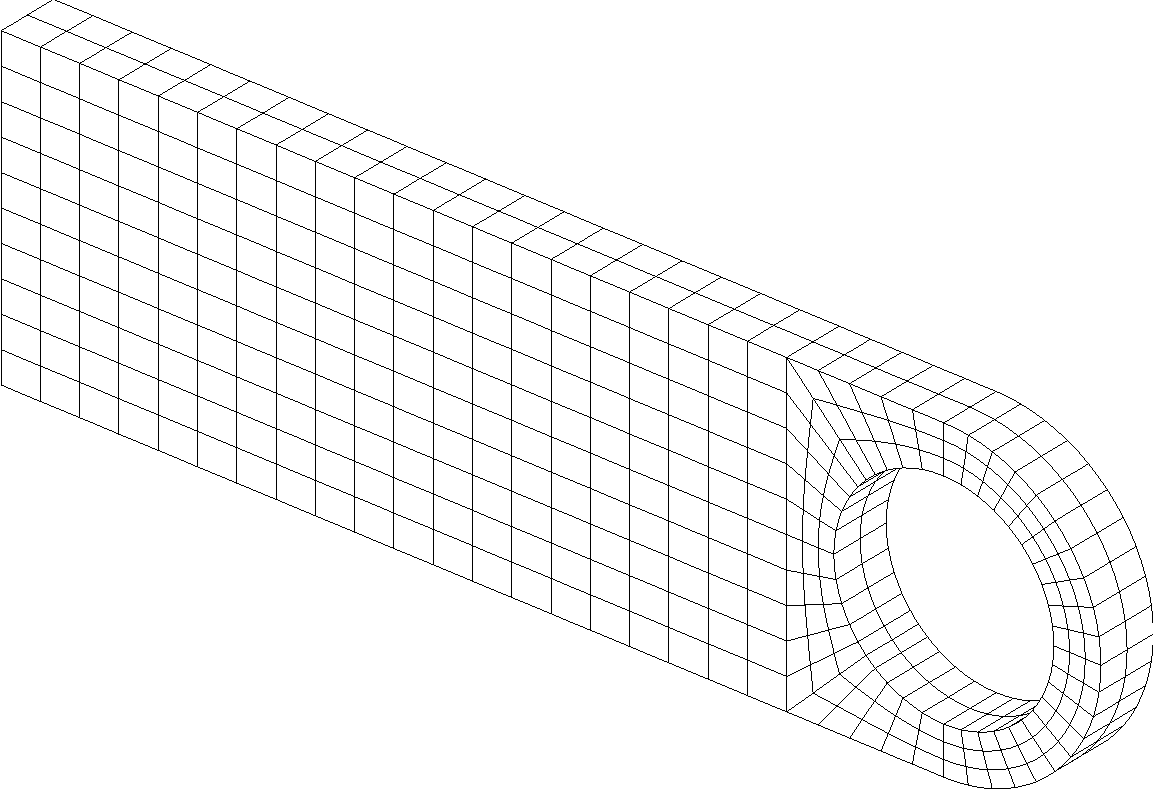
\includegraphics[width=4cm]{images/exo/1.2_maillage_hexa.4}
    \end{textblock*}
  \end{itemize}
\end{frame}

\begin{frame}{\fe{1.2 Maillage structuré}{1.2 Structured mesh}}
  \begin{itemize}
    \item \fe{Récupération de sous zones}{Subzone recovery}
    \lstinputlisting[language=gibiane, firstline=191, lastline=197]{dgibi/formation_debutant_1_maillage.dgibi}
    \item<2->\fe{Sauvegarde des données}{Saving data}
    \lstinputlisting[language=gibiane, firstline=215, lastline=218]{dgibi/formation_debutant_1_maillage.dgibi}
  \end{itemize}
\end{frame}
